\section{Descomposición bidimensional (por bloques 2D)}

\begin{figure}[H]
\centering
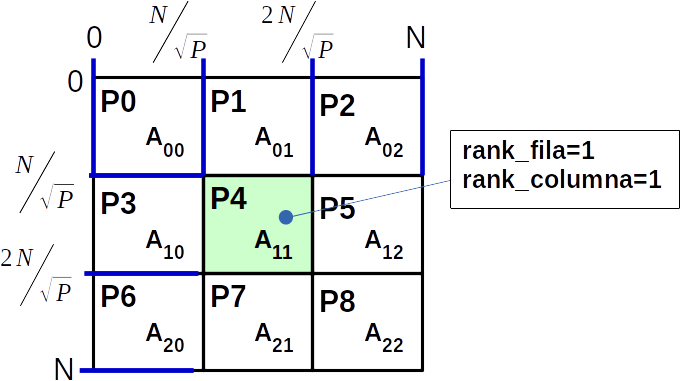
\includegraphics[width=0.8\textwidth]{imagenes/1.png}
\caption{Distribución por bloques 2D de la matriz \textit{A}}
\end{figure}

Este reparto de la matriz se hace empaquetando la matriz de la forma que ilustra la siguiente figura:

\begin{figure}[H]
\centering
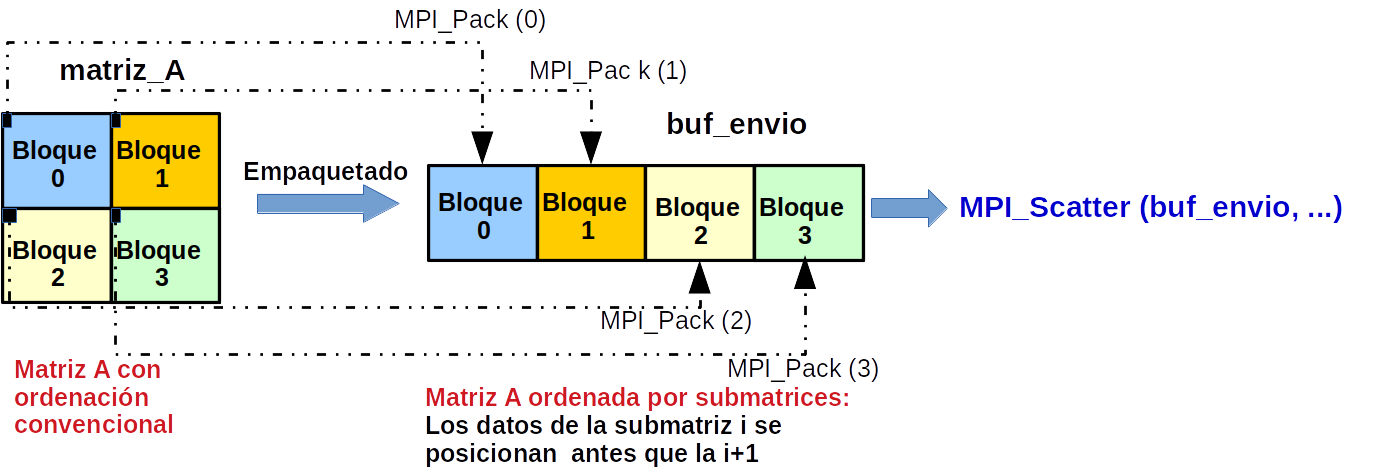
\includegraphics[width=0.8\textwidth]{imagenes/3.png}
\caption{Empaquetado de la matriz por bloques para p=4}
\end{figure}

\begin{figure}[H]
\centering
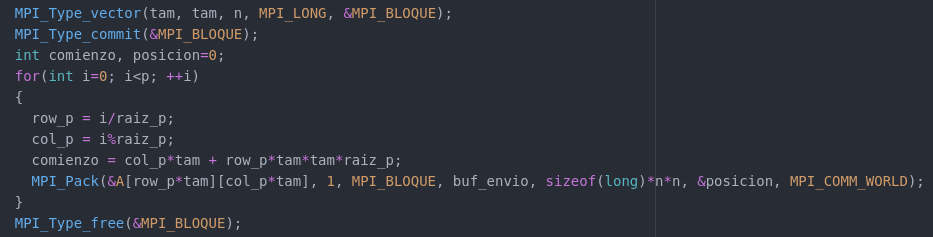
\includegraphics[width=0.8\textwidth]{imagenes/tipo.png}
\caption{Código para realizar el empaquetado de \textit{A}}
\end{figure}

Los comunicadores necesarios para la práctica se han obtenido de la siguiente manera.

\begin{figure}[H]
\centering
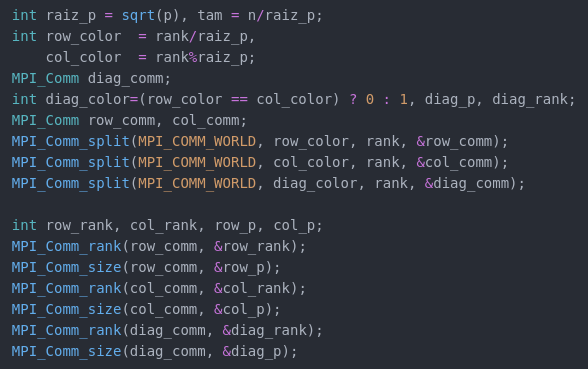
\includegraphics[width=0.8\textwidth]{imagenes/colores.png}
\caption{Obtención de los comunicadores necesarios}
\end{figure}

\begin{itemize}
\item \textit{Comunicador para las filas}: las partes enteras nos divide el comunicador en filas
\item \textit{Comunicador para las columnas}: el módulo nos divide a los procesadores en columnas con respecto a $\sqrt{P}$
\item \textit{Comunicador para la diagonal}: se divide dependiendo de si el comunicador para la fila y la columna coinciden.
\end{itemize}

Para repartir la matriz A, se realiza el siguiente \textit{scatter}.

\begin{figure}[H]
\centering
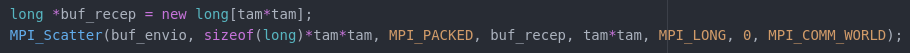
\includegraphics[width=0.8\textwidth]{imagenes/scatter-a.png}
\caption{Código del reparto de la matriz A en bloques2D}
\end{figure}

A continuación, se realiza el \textit{scatter} y el \textit{broadcast} de \textit{x} para obtener los elementos parciales, tal y como se indica en la siguiente figura:

\begin{figure}[H]
\centering
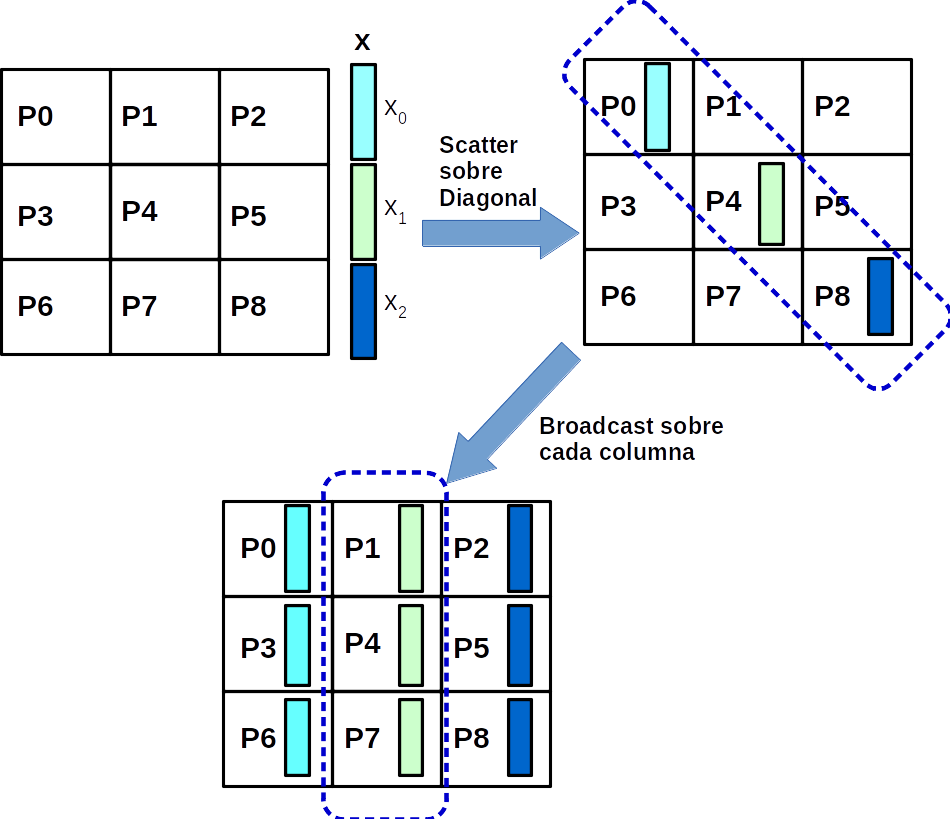
\includegraphics[width=0.8\textwidth]{imagenes/2.png}
\caption{Distribución de los subvectores del vector \textit{x} en una malla de ejemplo}
\end{figure}

\begin{figure}[H]
\centering
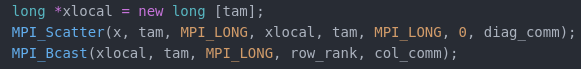
\includegraphics[width=0.8\textwidth]{imagenes/scatter-bcast-x.png}
\caption{Código que simula el comportamiento de la imagen anterior}
\end{figure}

Pasamos a calcular la parte que le corresponde del vector de salida y para cada proceso.

\begin{figure}[H]
\centering
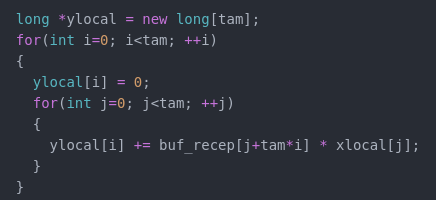
\includegraphics[width=0.8\textwidth]{imagenes/calculo-ylocal.png}
\caption{Código que calcula el segmento de \textit{y} correspondiente}
\end{figure}

Y finalmente, obtenemos las sumas locales(mediante reducción) y las reunimos en el proceso 0.

\begin{figure}[H]
\centering
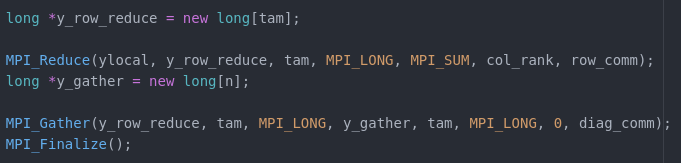
\includegraphics[width=0.8\textwidth]{imagenes/yfinal.png}
\caption{Código de la obtención de \textit{y}}
\end{figure}

Ejecución de ejemplo:

\begin{figure}[H]
\centering
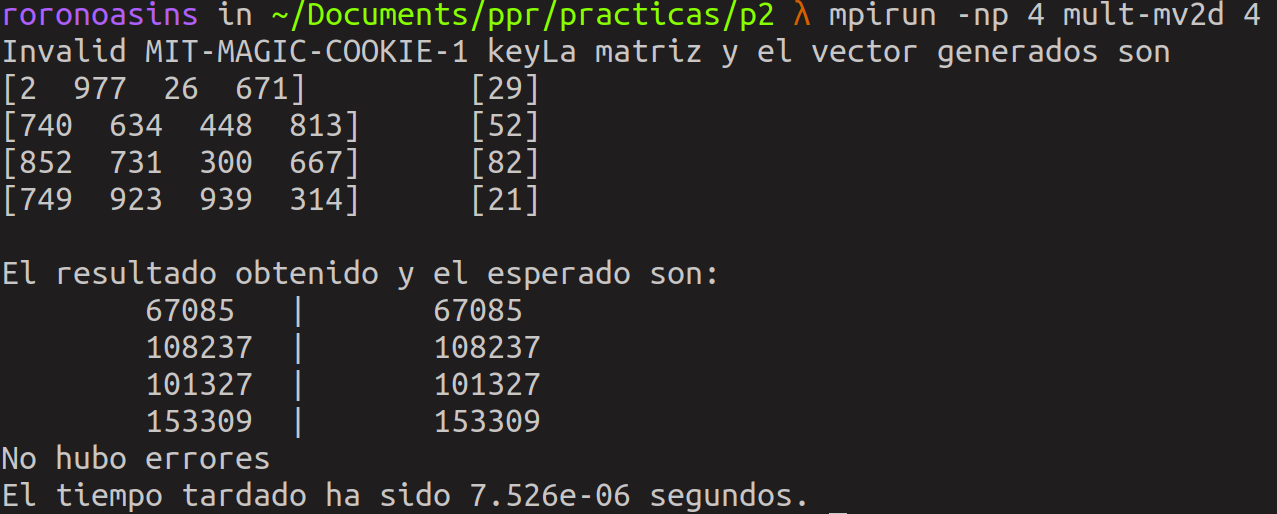
\includegraphics[width=0.8\textwidth]{imagenes/matrix.png}
\caption{Salida de ejemplo para una matriz 4x4 con p=4}
\end{figure}

Medición de los distintos ejercicios:

\begin{table}[H]
\begin{tabular}{ll|l|l|l|l|}
\cline{3-6}
                           &                                 & \multicolumn{2}{c|}{Unidimensional(bloques de filas)}    & \multicolumn{2}{c|}{Bidimensional(bloques 2d)}           \\ \hline
\multicolumn{1}{|c|}{N}    & \multicolumn{1}{c|}{secuencial} & \multicolumn{1}{c|}{P=4} & \multicolumn{1}{c|}{Ganancia} & \multicolumn{1}{c|}{P=4} & \multicolumn{1}{c|}{Ganancia} \\ \hline
\multicolumn{1}{|l|}{300}  & 0,000935                        & 0,000214529              & 4,35838511343455              & 0,0001501406             & 6,22749609366154              \\ \hline
\multicolumn{1}{|l|}{600}  & 0,002398                        & 0,000746907              & 3,21057373943476              & 0,0005137082             & 4,66801970457158              \\ \hline
\multicolumn{1}{|l|}{900}  & 0,0039364                       & 0,001480536              & 2,65876682498771              & 0,001214088              & 3,2422690941678               \\ \hline
\multicolumn{1}{|l|}{1200} & 0,0053216                       & 0,001930654              & 2,75637167509041              & 0,001607496              & 3,31049035269761              \\ \hline
\multicolumn{1}{|l|}{1400} & 0,008318                        & 0,002544616              & 3,26886257101268              & 0,001906264              & 4,3635089368524               \\ \hline
\end{tabular}
\end{table}

\begin{figure}[H]
\centering
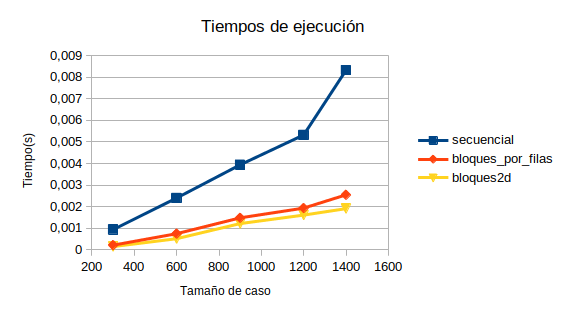
\includegraphics[width=0.8\textwidth]{imagenes/graphic.png}
\caption{Tiempos de ejecución obtenidos y ganancia}
\end{figure}

